\section{问题提出的背景}

\subsection{背景介绍}

在过去的十年里,深度学习已经逐渐成为了最主流的机器学习算法,并在图像处理、机器翻译、语音识别等诸多应用领域内取得了
巨大的成功。在机器学习算法中,深度神经网络凭借庞大的模型,通过训练巨大的数据和消耗极大的算力来达到在某些领域卓越
的精确度。然而这样的模型精度带来的推理计算复杂度代价是当下许多移动端、嵌入式设备无法承受的。那么针对移动边缘端设备
制定合适的深度神经网络就格外重要。

在以往的研究中,SqueezeNet\cite{iandola2016squeezenet}、Xception\cite{chollet2017xception}、
ResNeXt\cite{xie2017aggregated}、MobileNet系列\cite{howard2017mobilenets, sandler2018mobilenetv2}、
ShuffleNet系列\cite{zhang2018shufflenet,ma2018shufflenet}都针对边缘端设备内存较小、
计算能力相对服务端较弱的特性手工设计计算量相对较小的新颖的网络构造构造单元(分组卷积,深度可分离卷积等)。
这些网络都在维持了网络的特征提取能力和精度的基础上,极大地降低了网络的FLOPs(浮点运算操作数),
从理论上降低了网络的计算复杂度。而ShuffleNet V2\cite{ma2018shufflenet}在考虑了计算复杂度的同时
也考虑了内存访问代价,采取了使用输入输出数相同的卷积、消除分组卷积、减少网络分支数等措施,
取得了在近似FLOPs的条件下,Arm CPU和GPU推理延时小于先前业界最好模型的成果。
同时,这也指示了FLOPs作为一个理论指标,并不能被单一地用于评价特定模型在特定AI硬件上的计算复杂度。

除了网络结构的突破之外,近年来在移动边缘端设备上的神经网络推理平台、AI加速芯片都有卓越的进步。TensorFlow有配套的专为
移动端推理优化的TensorFlow Lite;PyTorch推出了Pytorch Mobile;近年来国内的边缘端推理引擎有腾讯的NCNN,
来自小米的MACE框架,百度的PaddlePaddle Lite,阿里巴巴的MNN等。除了软件之外,硬件平台也是百家争鸣:
高通骁龙SoC上除了ARM Cortex CPU、Adreno GPU之外还有采用VLIW(超长指令)架构的适合图像处理和神经网络计算的Hexagon DSP
(电子信号处理器);华为在2017年底推出了的Mate 10上搭载了寒武纪提供的全球第一款商用NPU(神经网络处理单元)Cambricon-1A,
这款芯片神经网络推理的性能与功耗比超过当年的旗舰CPU、GPU;最近Google推出的EdgeTPU,更是在八位整数推理MobileNet V2上达到了
接近400帧的速度;除此之外,Intel推出的Movidius计算棒,Rockchip(福州瑞芯微)推出的RK1808计算棒等,都会在
物联网、智慧城市等领域找到合适的落地场景大放异彩。

\subsubsection{项目提出的原因}

不论是在软件上还是在硬件上,神经网络推理平台表现出多样化,异构化的趋势。不同的硬件有截然不同的特性,在一种芯片
上能高效执行的网络不一定能很好地利用另一种芯片的硬件资源。如此看来,利用单一化的FLOPs作为衡量模型计算复杂度的指标来
指导设计神经网络是不合适的。那么针对多样化的软硬件寻找对应的合适的方法,设计高效的合适的神经网络就成为了重要的课题。
然而,不同的推理硬件可以搭配不同的推理软件,这样平方的组合数量就带来了平方级别的设计困难。
除此之外,``因地制宜''的网络设计过程往往会遭遇其他的困难,比如:硬件厂商通常不愿意提供详细的硬件设计信息;
许多AI芯片厂商提供的神经网络编译器、推理框架通常不会开源。这就给分析特定神经网络在特定AI芯片上的执行效率造成了极大地阻碍,
也进一步阻碍了为特定的AI芯片设计合适的神经网络。

本研究就在这样困难的背景下产生。本研究计划通过基准测试(Benchmark)的方式,测量多种神经网络构造单元在不同硬件下的
延时、效率(FLOPs/latency)表现,对比构造单元的理论复杂度,并结合已有的资料(开源代码、理论模型、可信的公开硬件架构信息等)
,分析理论复杂度和实际延时的差别,给``为异构硬件设计合适的神经网络''的目标提供实验数据和扎实的分析结果。

测量是理解和优化的关键。

\section{本研究的意义和目的}

\subsection{模型复杂度建模}
近年来神经网络结构搜索(NAS)成为了除了专家手工设计之外的设计神经网络的重要手段。当下的设计高效神经网络的NAS方案
通常采用混合精度和延时的目标函数作为优化目标,在特定硬件上搜索合适的网络。而评估延时往往会采用拟合
延时函数或者在目标机器上直接测量等的方式。
NasNet\cite{zoph2018learning}针对不同的计算量预算伸缩搜索空间;
MNasNet\cite{tan2019mnasnet}和MobileNet V3\cite{howard2019searching}直接在实机测量延时;
FBNet\cite{wu2019fbnet}采用了算子延时查找表和逐层累加延时的方式估算延时;
ProxylessNas\cite{cai2018proxylessnas}对逐层的算子构建了延时预测器预测延时。

这些方法都取得不错的效果,但是它们各自有各自的缺陷。针对不同计算量预算设计搜索空间需要人工的介入;
在实机测量延时并行度比较低而且成本巨大;使用延时查找表消耗庞大的存储空间;延时预测器不能精准地
理解硬件的特性,并且需要人工设计延时模型。本研究针对上述的缺陷,通过提供扎实的数据和分析结果,
可以帮助理解硬件的特性,启发设计更好的模型复杂度建模。

\subsection{性能数据驱动的模型优化方法}
因为边缘端AI加速器的兴起,所以设计边缘端友好的模型就相当重要。然而异构加速器厂商往往会使用闭源的编译器
和闭源的推理引擎,所以针对这样推理引擎的优化就变得困难且不现实。我们期望未来可以实现一个性能数据驱动的模型
优化方法,在图层次对模型进行优化。

\begin{figure}
    \begin{center}
        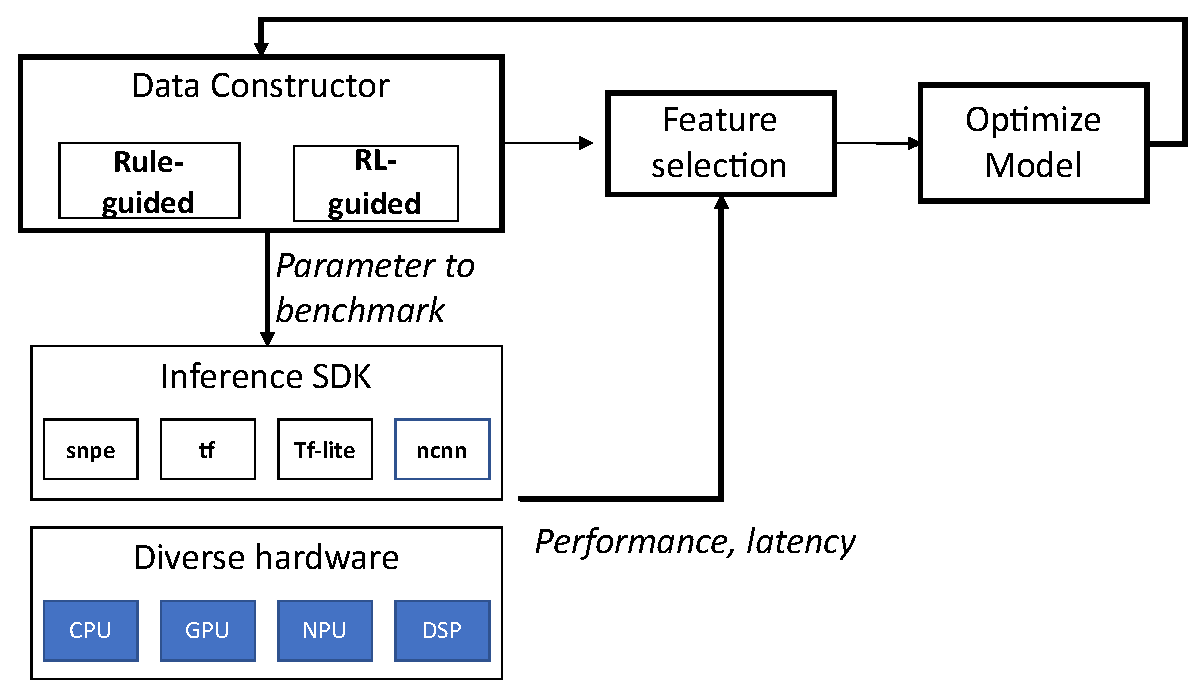
\includegraphics[width=0.9\textwidth]{figure/model_opt_sys.eps}
    \end{center}
    \caption{一个性能数据驱动的模型优化方法}
    \label{fig:model opt sys}
\end{figure}

由图\ref{fig:model opt sys}所示,该方法使用迭代式的优化方法。在每次迭代内,
一个控制器会利用强化学习或者规则导向的方法选择需要测量的测试点,根据选取的数据点在目标AI加速器上
测试获得性能数据,选择合适的有效的性能数据,再利用该数据对模型进行优化(比如修改某一层的通道数,或者内核大小),
在优化之后再利用控制器选择新的测试点。这样的方法的优势是可以针对黑盒的推理引擎进行优化。
而本研究就是为了更好的理解不同黑盒编译器和推理引擎的性能特征,为设计上述的控制器打下基础。